\documentclass[a4paper,11pt]{article}
\usepackage[left=1.5cm, right=1.5cm, top=2cm, bottom=1.5cm]{geometry}
\usepackage{graphicx}
\usepackage{amssymb}
\usepackage{amsmath}
\usepackage{wrapfig}

\begin{document}
\title{\LARGE{\textbf{ECEN 204 Design Report}\\Power Supply}}
\author{Niels Clayton : 300437590\\ \textbf{Lab Partner: }Nickolai Wolfe}
\date{September 15, 2019}
\maketitle
\hrule

\section{Introduction}
Most electrical devices require an external power supply in order to function.  In a New Zealand household, this power will be sourced from the 50Hz, 240V AC (alternating current) wall outlet. However most electrical devices require a much lower DC (direct current) voltage to operate correctly. To convert between this high voltage AC input and low voltage DC output a power supply can be used. This report will look at the aspects of a simple 12V AC to 5V DC power supply, and discuss possible design choices.

\subsection{Power Supply fundamentals}

\begin{figure}[h]
 \begin{center}
  \fbox{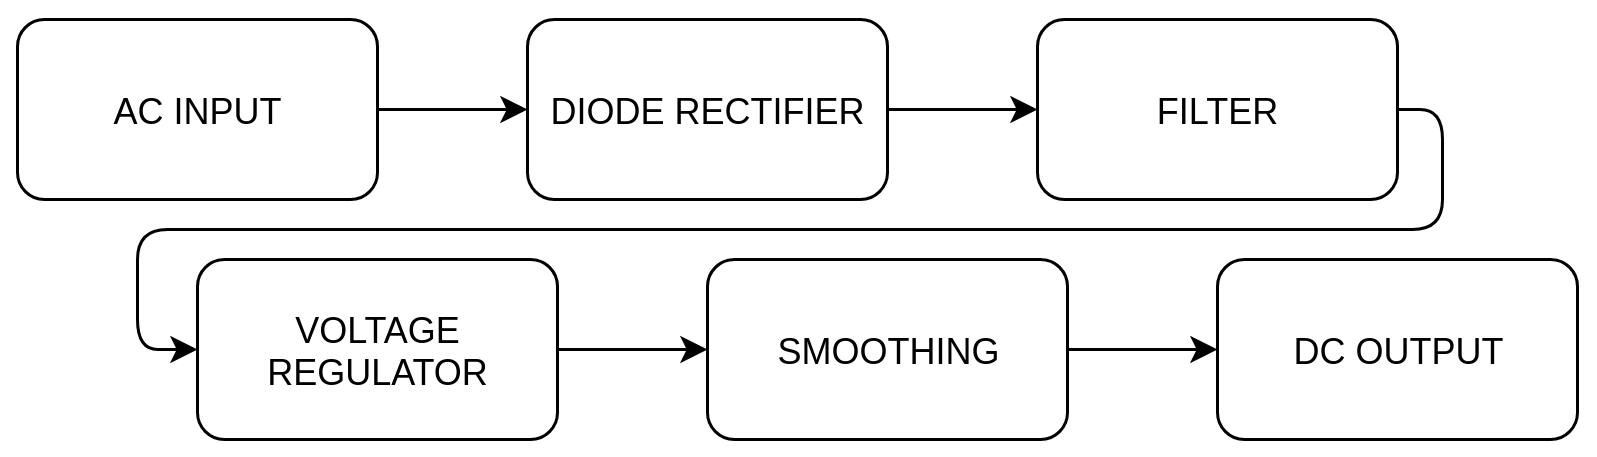
\includegraphics[width = \textwidth]{Images/Diagram.png}}
  \caption{Fundamental building blocks of a power supply}
 \end{center}
\end{figure}

Figure 1 shows the basic design of an AC to DC power supply, broken into the fundamental building blocks. The following section will expand upon the purpose of each of these. 

\subsubsection{AC Input}
The input voltage source for this projects power supply will be standard 240V, 50Hz AC. AC voltage oscillates as a sinusoidal signal, leading to both positive and negative currents. The AC input voltage will also need to be 'stepped down' to a lower voltage of 13.34V RMS (measured) using a transformer. This stepped down voltage is sufficiently close to the 12V input specified within this project.


\subsubsection{Diode Rectifier}
DC circuits are so labelled because they will not function correctly when supplied with an AC voltage. To deal with this, our AC input signal (figure 3) must be rectified to be a purely DC voltage (figure 4). This can be achieved using a rectifier circuit. 

There are three types of rectifier circuits, half-wave rectifiers, full-wave rectifiers, and centre-tapped transformer rectifiers. This design exercise will make use of the full-wave rectifier circuit, which will rectify both half waves of the input sinusoidal signal, compared to only half for the half-wave rectifier.

Diodes will only be conductive for one direction (polarity) of voltage, and can be observed to have near infinite impedance when place in the other direction. These states are knows are forward and reverse biased respectively. Due to this property of diodes, when arranged in the configuration showing in figure 2, a full-bridge rectifier circuit is created. This circuit works by only ever having two of the diodes forward biased at one time, providing only one path for current to flow regardless of input polarity. Because of this the output of the circuit will always be DC.

\begin{figure}[!htb]
\minipage{0.32\textwidth}
  \fbox{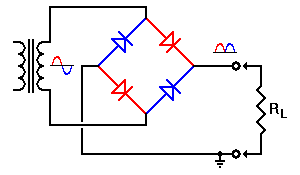
\includegraphics[width=0.99\textwidth]{Images/rectifier.png}}
  \caption{Full-bridge rectifier}
\endminipage\hfill
\minipage{0.32\textwidth}
  \fbox{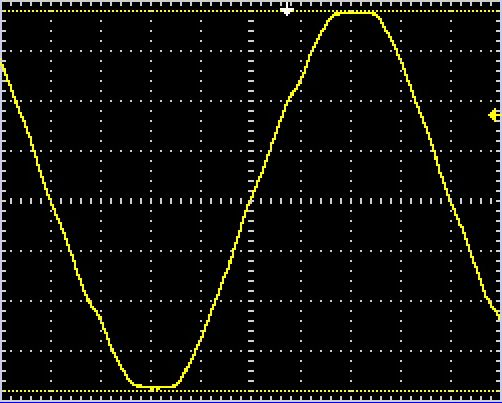
\includegraphics[width=\textwidth]{transformer_output.JPG}}
  \caption{AC input voltage}
\endminipage\hfill
\minipage{0.32\textwidth}%
  \fbox{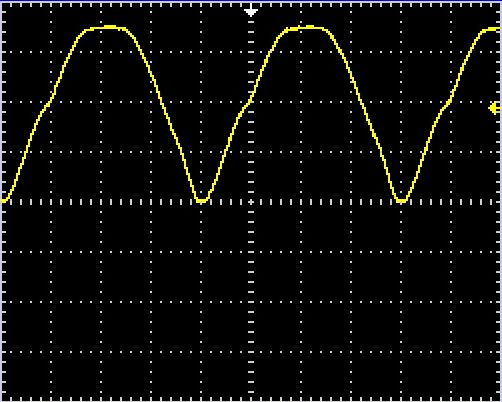
\includegraphics[width=\textwidth]{rectifier_output.JPG}}
  \caption{DC output voltage}
\endminipage
\end{figure}

\subsubsection{DC Filter}

For the output of our power supply we require a constant DC voltage. However after passing through the rectifier circuit the signal still resembles the original sinusoidal signal with large peaks and troths. In order to remedy this, the signal will be filtered.

Filtering is achieved by attaching a single capacitor between the the DC output and ground. This capacitor will charge while the voltage rises, and then discharge as the voltage begins to dip, effectively bridging the peaks of the input sinusoidal signal.

\begin{figure}[!htb]
\minipage{0.32\textwidth}
  \fbox{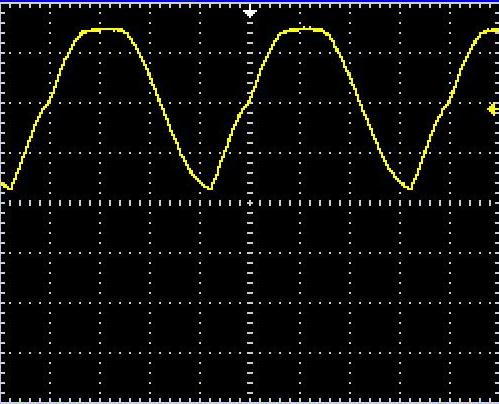
\includegraphics[width=0.98\textwidth]{Rectifier_out_different_cap_values/1uF_cap_rectifier1.JPG}}
  \caption{1uF capacitor}
\endminipage\hfill
\minipage{0.32\textwidth}
  \fbox{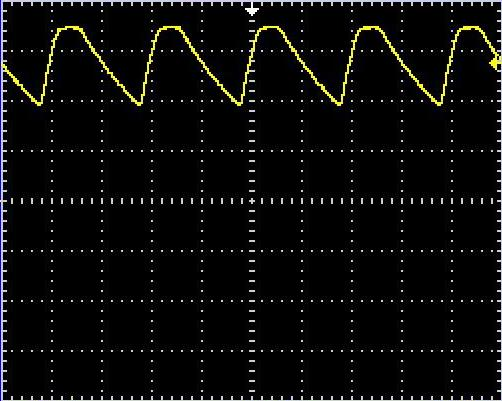
\includegraphics[width=0.98\textwidth]{Rectifier_out_different_cap_values/10uF_cap_rectifier1.JPG}}
  \caption{10uF capacitor}
\endminipage\hfill
\minipage{0.32\textwidth}%
  \fbox{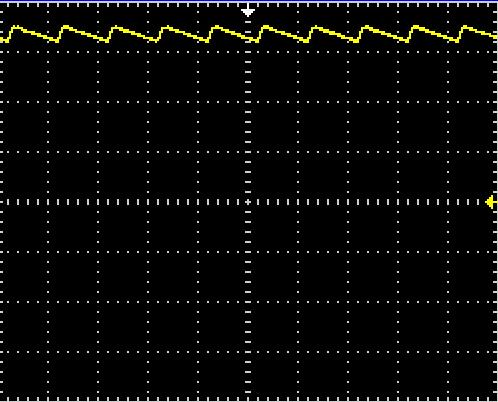
\includegraphics[width=0.98\textwidth]{Rectifier_out_different_cap_values/100uF_cap_rectifier1.JPG}}
  \caption{100uF capacitor}
\endminipage
\end{figure}

Figures 5, 6, and 7 show the output when filtered by different sized capacitors. As the size of the capacitor increases, more charge can be held by the capacitor, thereby filtering out more of the oscillation. It can be noted that it is only important to maintain a voltage above 6V, meaning that even the 10uF capacitor would be viable, however this is also load dependant.

\subsubsection{Voltage regulation and smoothing}

After Smoothing, a clean DC voltage will be output, however it will not be the required voltage and must be regulated to 5V. This can be achieved using zener diodes, linear voltage regulators, or a switch mode power supply. In this project we will use a linear voltage regulator as it will provide a more stable output as the load varies when compared to a zener diode, and its simplicity compared to the switch mode power supply.

However the linear voltage regulator does come with some trade-off's. Most notable are its limited current output, and its inefficiency. The input voltage to the regulator will be truncated, with all excess voltage being dissipated in the form of heat.

Finally the output of the regulator will have a second smoothing capacitor attached between it and ground. This capacitor functions very similarly the the filter cap, removing any irregularities in output voltage, but also serves to help with maintaining constant voltage with varying loads.

\section{Design}

The final design requirements specify the use of a L7805 5V linear voltage regulator, and 4 1N4007 diodes for rectification. Because of this, the voltage rectification and regulation methods are already predetermined. This allows us to select the filter and smoothing capacitors that will best fit our design requirements.
 
A selection of capacitors ranging from 1nF - 1000nF were tested for filtering the output of the rectifier (this is elaborated upon in the following section). It was concluded that a 10nF capacitor was sufficient for a 1k$\Omega$ load, however serious output ripple could be observed for loads lower than this. Because of this a filter capacitor size of 100nF was used in the final design. A capacitor of the same size was then chosen for output smoothing, This choice was made due to its relative unimportance in our use case of a static load, and for the simplicity of manufacturing. 

The major trade-off of this design is its efficiency. Our AC input was measured to have an RMS voltage of 13.34V, giving a DV voltage of 17.2V after rectification and smoothing. Given the design specifications of a 400mA max current through the transformer, and an output of exactly 5V DC, our regulator will have a calculated worst case efficiency of 29\%, dissipating a total of 4.8W. 

\begin{center}
\begin{tabular}{|c|c|c|c|c|c|}  
\hline
Voltage IN & Voltage OUT & Current IN/OUT & Power IN & Power OUT & Efficiency\\
\hline
8V & 5.2V & 9.63mA & 77mW & 50.1mW & 65\%\\
10V & 5.2V & 9.65mA & 96.5mW & 50.2mW & 52\%\\
12V & 5.2V & 9.68mA & 116mW & 50.3mW & 43.33\%\\
14V & 5.2V & 9.72mA & 136mW & 50.5mW & 37.14\%\\
\hline
\end{tabular}
\end{center}



\end{document}










\begin{wrapfigure}{r}{0.3\textwidth}
\fbox{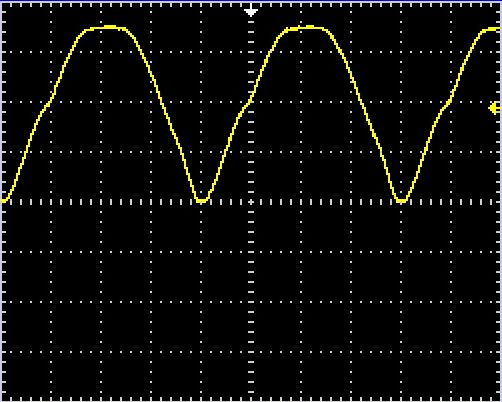
\includegraphics[width=0.3\textwidth]{rectifier_output.JPG}}
\caption{AC input voltage}
\end{wrapfigure}

\begin{figure}[!htb]
\minipage{0.32\textwidth}
  \fbox{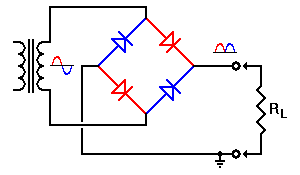
\includegraphics[width=0.3\textwidth]{Images/rectifier.png}}
  \caption{A really Awesome Image}
\endminipage\hfill
\minipage{0.32\textwidth}
  \fbox{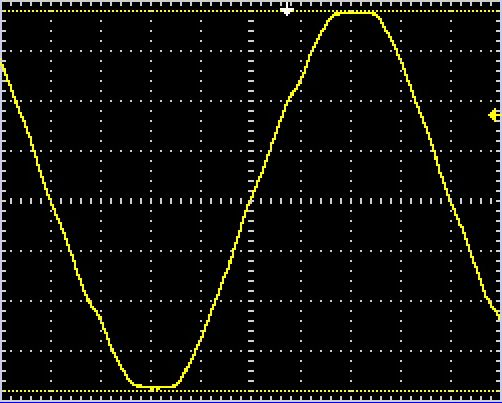
\includegraphics[width=0.3\textwidth]{transformer_output.JPG}}
  \caption{A really Awesome Image}
\endminipage\hfill
\minipage{0.32\textwidth}%
  \fbox{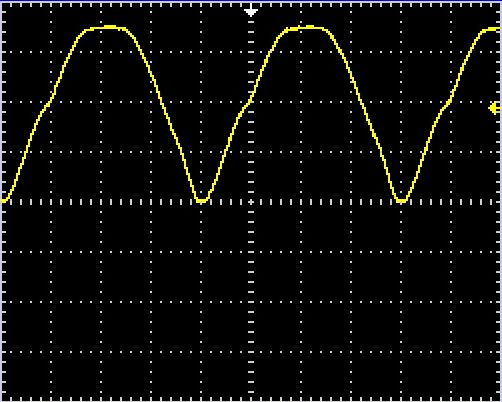
\includegraphics[width=0.3\textwidth]{rectifier_output.JPG}}
  \caption{A really Awesome Image}
\endminipage
\end{figure}